% 5. Prototyp (Implementierung, Patterns, Tests)
\chapter{Implementing the Modular Proxy Application}
\label{chap:implementation}
This chapter covers an exemplaric implementation of the monolithic concept that was worked out in section \ref{sec:design-1}, starting with formally describing the goals and constraints of this implementation in section \ref{sec:goals-constraints}. Afterwards, an overview and comparison of available and suitable tools for the task is performed in section \ref{sec:tool-selection}. The chapter concludes with details about the implementation of individual components in section \ref{sec:individual-components}, describing how specific challenges were overcome.% and what design patterns were used.

\section{Goals and Constraints}
\label{sec:goals-constraints}
The goal of this thesis' implementation was to implement the \enquote{Monolithic Proxy Application} design concept described in section \ref{sec:design-1} to a maturity level that allowed to test its usefulness and effectiveness in the testbed described in section \ref{sec:prototype-testing} that aimed to represent scenario \#2 discussed in section \ref{sec:example-scenarios}. Thus, a focus was set on implementing a vertical prototype that featured important core components (such as factories, state-machines and network stacks) and a set of exemplaric protocol implementations (\ac{HTTP}, \ac{WS} and \ac{MQTT}). Similar to the first prototype discussed in section \ref{sec:prototypical-implementation}, this prototype was a proof-of-concept implementation and neglected quality attributes such as usability and performance.\\
The prototype had the working title \enquote{net-riot}, which indicated that this was a networking tool and was to be used in the \ac{IoT} context. %While its core components and protocol implementations were successfully implemented and worked individually, the interoperation of of certain stacked \emph{IEncoder} implementations failed at runtime and could not be resolved before the end of this thesis.

\section{Tool Selection}
\label{sec:tool-selection}
To choose the tools for implementing the design concept, a list of requirements to tools was inferred from the software requirements discussed and expert interviews shown in chapter \ref{chap:understanding-the-problem-space}:
\begin{itemize}
    \item [\textbf{T1}] \textbf{Scripting:} The tool must provide scripting capabilities that allow penetration testers to execute complex scripted operations on messages.
    \item [\textbf{T2}] \textbf{Libraries:} In order to avoid custom implementation of the \ac{HTTP}, \ac{WS} and \ac{MQTT} protocols, the tool must provide a rich set of libraries that can be used to work with said protocols.
    \item [\textbf{T3}] \textbf{Deployment:} To allow the prototype to be installed in an uncomplicated way, the tool must provide or support mechanisms that simplify deployment, such as code compilation and static linking of dependencies or containerization.
    \item [\textbf{T4}] \textbf{Accessibility:} The tool must be powerful and complex enough to solve the software requirements and implement the design concept, but it must also feature a \enquote{barrier or entry} that is low enough so extending the application is feasible for open source developers.
\end{itemize}

Regarding the selection of a suitable programming language, it was found that Python satisfied all of these requirements:
\begin{itemize}
    \item Python is a free, open source and general purpose programming language that was first released in 1991 and is being continuously improved and updated. % 978-0-262-52962-4
    \item The built-in \emph{exec}\footnote{https://docs.python.org/3/library/functions.html\#exec} function provides execution of arbitrary Python code at runtime. Although it is infamous for its security implications, it is very suitable for scripting.
    \item The \ac{PyPI} is a public repository of more than 300.000\footnote{Based on \ac{PyPI}'s statistics: https://pypi.org/} Python packages that can be installed using the \emph{pip} command-line tool. There are numerous packages that implement the protocols \ac{WS}, \ac{MQTT} and \ac{HTTP}.
    \item Python supports multiple ways to deploy projects, including packaging projects into executable files \footnote{https://packaging.python.org/overview/\#bringing-your-own-python-executable} and containerization\footnote{e.g. using Docker https://hub.docker.com/\_/python/}.
    \item Its comparatively simple syntax and its design philosophy that values accessible code higher than performance\footnote{Described in 19 aphorisms in \enquote{The Zen of Python} (https://www.python.org/dev/peps/pep-0020/)} encourage readability and maintainability in Python projects. When implemented, this makes Python an accessible programming language. Also, its optional static typing allows to omit redundant type information for simple methods and to provide explicit type information for complex and shared pieces of code like algorithms and interfaces.
\end{itemize} %TODO: Python is free?
Git was used for version-control and Microsoft Visual Studio Code was the \ac{IDE} used for implementation.


\section{Individual Components}
\label{sec:individual-components}
The following sections discuss especially challenging aspects of net-riot's implementation, which problems were encountered and how they were solved.

\subsection{Gateways}
The protocols used in scenario \#2 (\ac{HTTP}, \ac{WS} and \ac{MQTT}) are used on top of \ac{TCP}. Therefore, net-riot implemented a \ac{TCP}-Gateway that allowed it to create \ac{TCP} server sockets to listen on for incoming connection requests. For incoming connections C\textsubscript{I}, respective outgoing connections C\textsubscript{O} were initialized and connected to a preconfigured remote server. For each of those connections, \enquote{TcpPipe} instances P\textsubscript{I} and P\textsubscript{O} were initialized that ran in separate threads and accepted incoming packets. The gateway then initialized \enquote{TcpGatewayPipe} instances with P\textsubscript{I} and P\textsubscript{O} that routed messages originating from the TcpPipes into the pipeline and from the pipeline to the correct TcpPipe instance.\\
Messages that originated from gateways were temporarily stored in a queue so that only a single message was processed in the pipeline at any given time. It was found that if multiple messages were processed simultaneously, the global state-machine could change states while a message was still being processed in a then inactive state, resulting in this state's network stack being left unconnected and unable to route the message back up the pipeline. For the same reason, net-riot only supported one single connection.


\subsection{Encoders}
For each of the protocols used in scenario \#2, net-riot implemented a separate IEncoder.
\paragraph{HttpEncoder} For \ac{HTTP}, no library was found that parsed \ac{HTTP} requests or responses into low-level representations that did not discard essential information. However, since \ac{HTTP} is a comparatively simple, text-based and stateless protocol, a custom IEncoder was implemented that parsed \ac{HTTP} requests and responses from raw binary data and allowed to assemble requests and responses from processed messages. For assembly, the implementation used the \ac{HTTP} header information contained in a message's \enquote{history} field that held the headers that were parsed when the message was first parsed by this encoder. One practical pitfall of the custom implementation was the \enquote{Content-Length} \ac{HTTP} header that indicated the number of bytes contained in an \ac{HTTP} request body or \ac{HTTP} response body. Systems that parse \ac{HTTP} messages (such as web-servers and browsers) use the value of the \enquote{Content-Length} header to read the indicated number of bytes from a \ac{TCP} stream and associate it with the parsed headers. If the length of a message body is modified by a proxy, the \enquote{Content-Length} header indicates the wrong number of bytes to read: this will either result in reading too few bytes (thus, discarding information) or reading too many bytes rendering future requests malformed. To solve this issue, the custom encoder provided the configurable flag \emph{recalculateContentLength} that, if set to true, dynamically calculated the value of the \enquote{Content-Length} header to reflect the actual length of bytes contained in the message's BinarySource.
\paragraph{WsEncoder} The library used for \ac{WS} implementation was \enquote{websockets}\footnote{https://github.com/aaugustin/websockets/, commit 6b5cbaf41cdbc9a2074e357ccc613ef25517dd32}. It offered methods for parsing (\emph{framing.Frame.read}) and assembling (\emph{framing.Frame} constructor) \ac{WS} frames. These functions worked fine for regular \ac{WS} frames. However, to save bandwidth, some \ac{WS} client and server implementations make use of \ac{PMCE}. The use of \ac{PMCE} is indicated by the \enquote{rsv1} bit of \ac{WS} headers being set to true. While the library implemented \ac{PMCE} (\emph{extensions.permessage\_deflate.PerMessageDeflate}) and using the extension worked on the first messages of a \ac{WS} connection, it would fail to correctly compress messages after it processed a number of messages, causing the remote \ac{WS} clients and servers to terminate the connection. It was found that the \ac{PMCE} implementation was stateful and not reset after being used. This issue was solved by initializing new \emph{PerMessageDeflate} instances per \ac{WS} frame assembly.
\paragraph{MqttEncoder} For (de-)serialization of \ac{MQTT} messages, the library \enquote{hbmqtt}\footnote{https://github.com/beerfactory/hbmqtt/, commit 31165fb0e827925417f99a7b1f475a9d67e1c72f} was used in net-riot. The library implemented individual classes for each \ac{MQTT} message type and provided methods for parsing (\emph{from\_stream}) and assembly (\emph{to\_bytes}) of packets. However, the library did not provide any method that chose the correct class for (de-)serialization of a given binary buffer or processed message. Therefore, this functionality was implemented in net-riot: the \emph{MqttEncoder} defined a dictionary that mapped \ac{MQTT} message types to a tuple of classes (\emph{Packet}, \emph{VariableHeader} and \emph{Payload}) provided by the library and attempted to parse the basic \ac{MQTT} message header of a binary buffer. This header included the \ac{MQTT} message type that was then used to look up the correct classes for parsing in the dictionary. When \ac{MQTT} messages were re-assembled by the \emph{MqttEncoder}, it extracted the message type from the parsed header (that was stored in the message's \enquote{history} field) and used this to look up the correct classes for serialization in the dictionary.

%\lstinputlisting[firstline=2,language=Python,caption={Crypter-Interface},label=lst:CrypterInterface]{\srcloc/mqtt-encoder.py}

\subsection{Scripting}
In order to allow execution of scripts on messages, net-riot implemented the \enquote{ScriptProcessor} discussed in section \ref{sec:design-1}. This IProcessor implementation used Python's built-in \emph{exec} function for executing arbitrary Python code (shown in listing \ref{lst:ScriptProcessor}). The function allows the caller to define the available objects of the local and global scopes in the called code. This mechanism was used to pass the message instance, processing direction, context and \enquote{result} object to the script in the local scope. The \emph{ProcessingResult} values were passed to the script in the global scope which allowed to script to assign one of these values to the \enquote{result} object in the local scope. After execution, the \enquote{result} value was evaluated and returned by the ScriptProcessor. This effectively enabled scripts to:
\begin{itemize}
    \item Read and write fields and payloads of messages.
    \item Read and write the active pipeline's context and thus, its state-machines' memory. This could be used to trigger state transitions.
    \item Control whether messages were processed further, being immediately sent back up the pipeline, being dropped or ignored.
\end{itemize}
\lstinputlisting[language=Python,caption={The ScriptProcessor implementation of net-riot using Python's built-in exec function.},label=lst:ScriptProcessor]{\srcloc/scriptprocessor.py}
For net-riot to support \ac{MQTT} communication that was tunnelled via \ac{WS} it had to detect upgrades of \ac{HTTP} connections to \ac{WS}. This was achieved by ScriptProcessor instances that executed scripts that examined the \ac{HTTP} communication and set values in the memory of specific state-machines using the context that was supplied to them. Listing \ref{lst:UpgradeScript} shows the script that detected a server's \ac{HTTP} response to an upgrade to \ac{WS}: if there was an \enquote{Upgrade} header with the value \enquote{websockets} and if the status code of the response was $101$, the key \enquote{serverUpgrade} of the nested state-machine \enquote{http} was set to $True$. If any of these checks failed, it was set to $False$. This script worked in conjunction with another script that performed similar checks to detect a client's request to upgrade the connection. The \enquote{http} state-machine used \enquote{ScriptRules} that evaluated the value of the \enquote{serverUpgrade} key and triggered a state transition if both a client's upgrade request and the server's upgrade response were detected.
\lstinputlisting[language=Python,caption={The script net-riot used to detect upgrades of \ac{HTTP} connections to \ac{WS}.},label=lst:UpgradeScript]{\srcloc/script.py}

\subsection{Configuration Parsing and Building}
The requirement \enquote{F2 Network Stacks} mandated the capability to read a configuration file at runtime and initialize the therein specified hierarchy of state-machines and network stacks.

\paragraph{JSON Configuration and Schemas} For formal specification and representation of state-machines and network configurations, net-riot made use of the \ac{JSON} format. In over 600 lines of code, a \ac{JSON} schema was defined that specified the structure and types of net-riot configuration files. \ac{JSON} and \ac{JSON} schema were chosen over alternatives such as XML and YAML due to their simple syntax, flexibility and powerful features (such as $definitions$).

% Schema: definitions, flat hierarchy
\paragraph{Factories, Builders and Templates}

\begin{figure}[h]
    \centering
    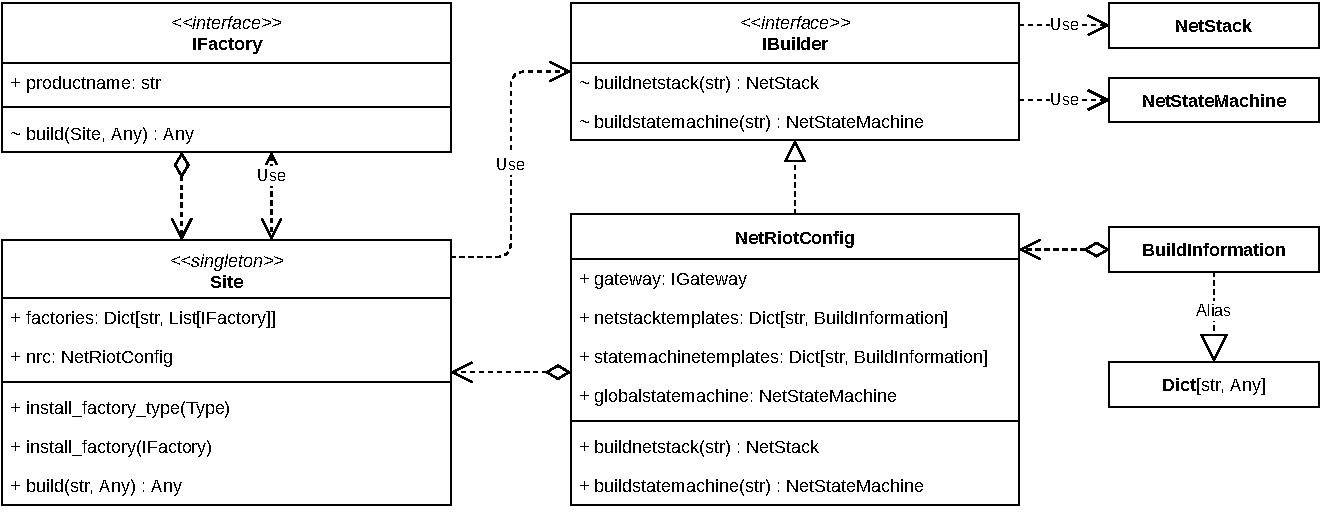
\includegraphics[width=14cm]{img/ch06/net-riot-factory.pdf}
    \captionof{figure}{?} %TODO: Describe
    \label{fig:net-riot-factory}
\end{figure}
% Site + NetRiotConfig + Templates + Reflection
The \enquote{Site} component was briefly discussed in section \ref{sec:design-1} and envisioned as an implementation of the abstract factory pattern. Figure \ref{fig:net-riot-factory} shows net-riot's implementation of the Site component and its associated interfaces and classes. The Site component holds a dictionary that maps product-names to factories. In turn, factories can instantiate objects such as pipes, gateways and state-machines (each differentiated by distinct names). Listing \ref{lst:ScriptRuleFactory} shows a simple factory implementation that is used to instantiate \enquote{ScriptRule} objects. However, prior to calling the constructor of the ScriptRule class, it needs to acquire a \enquote{Script} instance. It does so by requesting the Site to build a Script instance with the supplied information. In turn, the Site looks up the correct factory to use for instantiating the requested Script instance and calls it. Thus, factories can recursively request further objects to be built by the Site while they themselves provide the functionality to produce a single product each.
\lstinputlisting[language=Python,caption={A simple factory that requested the build of a \enquote{Script} instance to instantiate a \enquote{ScriptRule}.},label=lst:ScriptRuleFactory]{\srcloc/scriptrulefactory.py}
The \enquote{NetRiotConfig} class implements further logic to net-riot that allows to dynamically instantiate whole state-machines and network stacks. It does so by saving the configured state-machines and network stacks as \emph{templates} and passing them to the Site to build. For instance, net-riot's configuration file may specify a state-machine by the name of \enquote{http\_to\_ws} that is specified to be used as a nested \ac{FSM} of a state \enquote{entry} of the global state-machine. When the global state-machine is built and an instance of the nested \ac{FSM} is requested, the Site component calls NetRiotConfig's \emph{buildstatemachine} method and supplies the name \enquote{http\_to\_ws}. In turn, NetRiotConfig calls the Site component's \emph{build} function and supplies the template of the requested state-machine.\\
Also, net-riot used Python's \enquote{inspect} package to dynamically acquire all types of implemented factories and register them in the Site instance (shown in listing \ref{lst:Reflection}).

\lstinputlisting[language=Python,caption={Dynamic registering of all factory implementations.},label=lst:Reflection]{\srcloc/load_factories.py}

%TODO : CLI?